\chapter{Configuring iSCSI Target and Initiator}

\section{Understanding iSCSI Target and Initiator}
\textbf{SCSI (Small Computer System Interface)} [read as \textit{scuzzy}] is an alternative to ATA (a.k.a. IDE) Hard drives, which most consumer computers stick to. While SCSI drives provide significantly more throughput for certain scenarios, IDE suffices for most home computer usage. However, in case of servers, SCSI proves to be a much better alternative, since they provide more reliability and data transfer speed (much higher than ATA), owing to the fact that data transfer occurs in full-duplex mode (i.e., data can be read and written at the same time at full speeds). They also boast higher speeds (such as 15,000 RPM) as compared to ATA speeds (7200 RPM). Another reason servers tend to use SCSI (or related technologies, such as Serially Attached SCSI or SAS) is that the protocol makes it easy to \textit{daisy-chain} several SCSI devices to the same controller, several times that of IDE devices. In fact, in the pre-USB era, SCSI was the go-to common interface for connecting peripherals or even devices such as printers. 

Traditional SCSI devices use a long cable and a SCSI \textbf{Command Descriptor Block (CDB)} command to interact with the SCSI devices. In case of iSCSI, the same CDBs are used, but they're transmitted over IP packets over a network, instead of the cable. Thus, the SCSI devices are emulated by using a storage backend and presenting them on the network using iSCSI targets. SCSI targets are typically storage devices, while the hosts they're connected to are the initiators. Thus, this technology enables us to share PVs or LVs on the network, represented by iSCSI targets. 

A \textbf{Storage Area Network (SAN)} is a network that provides access to a consolidated, block level data storage. \textit{Block devices} provide a buffered data storage method, where data is transferred from the kernel buffer to the physical device. Also, data can be read and written in entire blocks. SANs thus present devices such as disk arrays as locally attached storage to servers. \textbf{Fiber Channel} or \textbf{FC} is a high speed network technology developed to enable fast data transfers between servers and SANs. Ethernet structures utilizing iSCSI technology can be as fast as their FC structure counterparts, thus making the technology enterprise ready for SAN creation. 

\subsection{iSCSI Operation}
In the case of iSCSI storage, we have the SAN, on which runs a \textit{iSCSI target} which can provide access to the storage backend. For any server that needs to access the files hosted by the SAN, it needs to run an \textbf{iSCSI initiator}, which performs a discovery operation first. During this, the SAN tells it about the iSCSI devices it has to offer. Once this is complete, the iSCSI initiator can login to the devices.


\subsection{iSCSI Components}
Both the iSCSI targets and the storage backends need to be set up for the SAN to operate. The storage backend can be an entire disk, a dedicated partition, a logical volume or even a file! The servers, running the iSCSI initiators, will see the iSCSI targets as new storage devices after successfully logging in to them. This can be verified by viewing the output of the \verb|/proc/partitions| file. A tool called \textit{lsscsi} can also alternatively used, although it is not installed by default. 

\subsection{Basic iSCSI Terminology}
\noindent
\begin{tabular}{rM{0.85}}
	\toprule
	\textbf{Terms} &\textbf{Description} \\
	\midrule
	\textbf{IQN}	&iSCSI Qualified Name - an unique name assigned to each iSCSI target and initiator, used to identify them.\\
	\textbf{Initiator}	&The iSCSI client that is identified by its IQN.\\
	\textbf{Target}	&The service on the iSCSI server that gives access to the storage backend.\\
	\textbf{ACLs}	&Access Control Lists that are based on the node's IQNs.\\
	\textbf{Portal}	&Also known as \textbf{nodes}, this is the combination of the IP address and the port that are used by both targets and initiators to establish connections.\\
	\textbf{discovery} &The process through which an indicator finds the available targets that are configured for a given portal.\\
	\textbf{LUNs} &The \textit{Logical Unit Number} is a number used to identify the logical unit (i.e., block devices shared through the target) being addressed by the iSCSI Controller.\\
	\textbf{login} &The act which gives an initiator the relevant LUNs.\\
	\textbf{TPG} &The \textit{Target Portal Group} is a collection of IP Addresses and TCP ports to which a particular iSCSI Target will listen.\\
	\bottomrule
\end{tabular}

\noindent
So, there can be more than one portals per server, and more than one targets per portal. 

\subsection{After connecting an initiator to an iSCSI Target}
The new block devices thus accessed will appear as local devices (/dev/sdb, /dev/sdc etc.) Note that if a LUN is available and used by multiple servers, multiple devices can access the LUN post connection, i.e., multiple servers can use the disk at the same time. This is a bit dangerous, since it requires using clustering, for providing multiple servers to use the storage. Otherwise for a file system like XFS or Ext4, two servers writing to the same file can cause data loss. 

To avoid this, shared file systems such as GFS2 can be used. In GFS2, the file system cache is shared among all the nodes. Thus, all nodes writing to the file system know what all the other nodes are doing. 

\section{Setting up an iSCSI Target}
The iSCSI target works with several storage backend devices on the SAN. These storage devices can be anything that can be used for PVs when using traditional LVM. All these devices are put together in a volume group, which is then subdivided into several LVs. These LVs are each assigned a LUN. 

\begin{figure}[H]
	\centering
	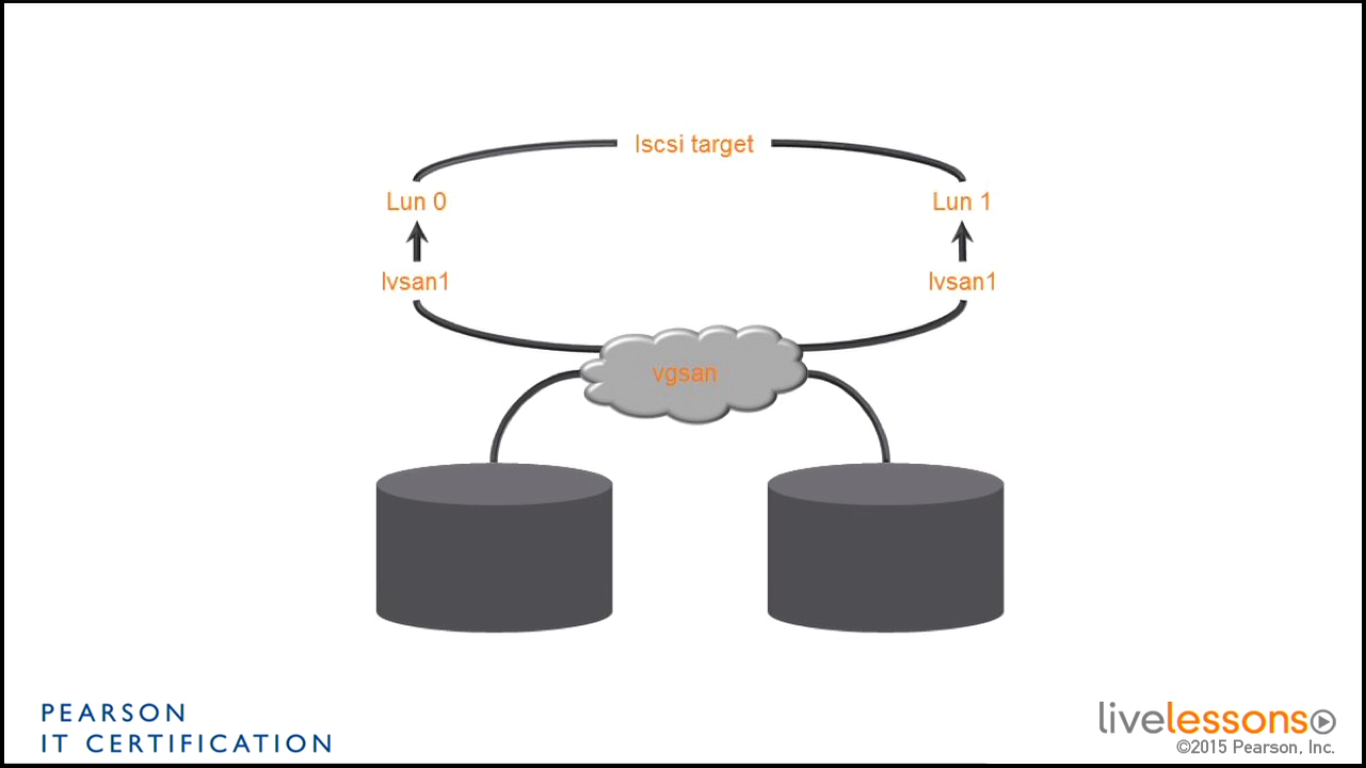
\includegraphics[width=0.9\linewidth]{Mod1/chapters/1.2.a}
	\caption{iSCSI Target Setup}
	\label{fig:1 iSCSI Target Setup}
\end{figure}

\noindent
These LUNs are presented using the iSCSI targets. Thus, the iSCSI configuration is created on top of a traditional LVM configuration. 

\subsection{Creating the LVM}
Let us consider we have an empty disk of 1GB on which we want to build the iSCSI configuration. This can be verified using:

\vspace{-15pt}
\begin{minted}{console}
# lsblk
NAME            MAJ:MIN RM  SIZE RO TYPE MOUNTPOINT
sda               8:0    0   20G  0 disk 
├─sda1            8:1    0    1G  0 part /boot
└─sda2            8:2    0   19G  0 part 
├─centos-root 253:0    0   17G  0 lvm  /
└─centos-swap 253:1    0    2G  0 lvm  [SWAP]
sdb               8:16   0    1G  0 disk 
sr0              11:0    1  8.1G  0 rom  
\end{minted}
\vspace{-10pt}

\noindent
We can directly create the VG \verb|vgsan| on it, using:

\vspace{-15pt}
\begin{minted}{console}
# vgcreate vgSAN /dev/sdb
Physical volume "/dev/sdb" successfully created.
Volume group "vgSAN" successfully created
# pvs
PV         VG     Fmt  Attr PSize    PFree   
/dev/sda2  centos lvm2 a--   <19.00g       0 
/dev/sdb   vgSAN  lvm2 a--  1020.00m 1020.00m
# vgs
VG     #PV #LV #SN Attr   VSize    VFree   
centos   1   2   0 wz--n-  <19.00g       0 
vgSAN    1   0   0 wz--n- 1020.00m 1020.00m
\end{minted}
\vspace{-10pt}

\noindent
The output of the \verb|pvs| and \verb|vgs| commands show that the PV \verb|/dev/sdb| is now a part of \textit{vgSAN}, which has a free space of 1020MB. Now we create two LVs \textit{lvSAN1} and \textit{lvSAN2} on the VG, using:

\vspace{-15pt}
\begin{minted}{console}
# lvcreate -L 500M -n lvSAN1 vgSAN
Logical volume "lvSAN1" created.
# lvcreate -l 100%FREE -n lvSAN2 vgSAN
Logical volume "lvSAN2" created.
# lvs
LV     VG     Attr       LSize   Pool Origin ... Convert
root   centos -wi-ao---- <17.00g                                                    
swap   centos -wi-ao----   2.00g                                                    
lvSAN1 vgSAN  -wi-a----- 500.00m                                                    
lvSAN2 vgSAN  -wi-a----- 520.00m                                                    
\end{minted}
\vspace{-10pt}

\noindent
Now, our LVM setup is complete, and we can proceed with the iSCSI setup. For this, first of all we need to install the iSCSI software, called \textbf{targetcli}. The targetcli utility is a relatively new one capable of managing multiple types of storage devices. 

\subsection{Creating the iSCSI configuration using targetcli}
We start the utility using:

\vspace{-15pt}
\begin{minted}{console}
# targetcli
Warning: Could not load preferences file /root/.targetcli/prefs.bin.
targetcli shell version 2.1.fb46
Copyright 2011-2013 by Datera, Inc and others.
For help on commands, type 'help'.

/> 
\end{minted}
\vspace{-10pt}

\noindent
This interface can be navigated using the same commands as the bash shell. Using the \verb|cd| command produces the output:

\vspace{-15pt}
\begin{minted}{console}
/> ls
o- / ..................................................................... [...]
  o- backstores .......................................................... [...]
  | o- block .............................................. [Storage Objects: 0]
  | o- fileio ............................................. [Storage Objects: 0]
  | o- pscsi .............................................. [Storage Objects: 0]
  | o- ramdisk ............................................ [Storage Objects: 0]
  o- iscsi ........................................................ [Targets: 0]
  o- loopback ..................................................... [Targets: 0]
/> 
\end{minted}
\vspace{-10pt}

\noindent
The \textit{backstores} part allow us to work with the different storage devices. To enter backstores, we simply enter \verb|cd| command, and select it from the menu. This will change the prompt to \verb|/backstores>|. Here, we can see it contains the \textit{block}, the \textit{fileio}, the \textit{pSCSI} and the \textit{ramdisk} devices. Their significance is explained below:

\noindent
\begin{tabular}{rM{0.83}}
	\toprule
	\textbf{Types} &\textbf{Description} \\
	\midrule
	\textbf{Block}	&Refers to any block device that we want to share using iSCSI. This includes all traditional disks, partitions and even LVMs.\\
	\textbf{fileio}	&Refers to a file that can be used as a storage source. This refers to a big file created using a tool such as \verb|dd|.\\
	\textbf{pscsi}	&Physical SCSI - a SCSI pass-through backstore is created for such devices.\\
	\textbf{ramdisk}	&RAM storage, wiped with every reboot, and is thus a \textbf{very} bad idea.\\
	\bottomrule
\end{tabular}

\noindent
Now, since all our LVs are block devices (by their very nature), we have to create our LUNs inside the block category. This we can do using:

\vspace{-15pt}
\begin{minted}{console}
/backstores> block/ create block1 /dev/vgSAN/lvSAN1
Created block storage object block1 using /dev/vgSAN/lvSAN1.
\end{minted}
\vspace{-10pt}

\noindent
The command instructs the targetcli utility to enter the block category, and create a block device called \textit{block1} from the \verb|/dev/vgSAN/lvSAN1| device. We can create another block device for the partition and a 1G custom file device using:

\vspace{-15pt}
\begin{minted}{console}
/backstores> block/ create block2 /dev/vgSAN/lvSAN2
Created block storage object block2 using /dev/vgSAN/lvSAN2.
/backstores> fileio/ create file1 /root/diskFile1 1G
Created fileio file1 with size 1073741824
\end{minted}
\vspace{-10pt}

\noindent
When creating a file, we can merely specify the size (1GB) and the name \& location (/root/diskFile1) to have the \verb|targetcli| utility create the file for us, instead of copying from \verb|/dev/zero| to a file using \verb|dd|. All the different devices thus added can be seen with:

\vspace{-15pt}
\begin{minted}{console}
/backstores> ls
o- backstores ............................................................ [...]
  o- block ................................................ [Storage Objects: 2]
  | o- block1 ............ [/dev/vgSAN/lvSAN1 (500.0MiB) write-thru deactivated]
  | | o- alua ................................................. [ALUA Groups: 1]
  | |   o- default_tg_pt_gp ..................... [ALUA state: Active/optimized]
  | o- block2 ............ [/dev/vgSAN/lvSAN2 (520.0MiB) write-thru deactivated]
  |   o- alua ................................................. [ALUA Groups: 1]
  |     o- default_tg_pt_gp ..................... [ALUA state: Active/optimized]
  o- fileio ............................................... [Storage Objects: 1]
  | o- file1 ................. [/root/diskFile1 (1.0GiB) write-back deactivated]
  |   o- alua ................................................. [ALUA Groups: 1]
  |     o- default_tg_pt_gp ..................... [ALUA state: Active/optimized]
  o- pscsi ................................................ [Storage Objects: 0]
  o- ramdisk .............................................. [Storage Objects: 0]
\end{minted}
\vspace{-10pt}

\noindent
Now that the block devices are ready, we can go to the \verb|/iscsi| environment and prepare the iSCSI targets. Initially, there will be no targets:

\vspace{-15pt}
\begin{minted}{console}
/backstores> cd /iscsi
/iscsi> ls
o- iscsi .......................................................... [Targets: 0]
\end{minted}
\vspace{-10pt}

\subsection{Target Creation}
Now, we create a target that provides access to the backing storage devices called \textit{block1}, \textit{block2} and \textit{file1}. This can be done using the \verb|create| command, followed by an IQN. IQNs are typically created using a naming format: $$\verb|iqn.<yearOfCreation>-<monthOfCreation>.<reverseDomainName>:<targetName>|$$ Thus, ours will be named: \verb|iqn.2018-01.local.somuvmnet:target1|. This can be done with:

\vspace{-15pt}
\begin{minted}{console}
/iscsi> create iqn.2018-01.local.somuvmnet:target1
Created target iqn.2018-01.local.somuvmnet:target1.
Created TPG 1.
Global pref auto_add_default_portal=true
Created default portal listening on all IPs (0.0.0.0), port 3260.
\end{minted}
\vspace{-10pt}

\noindent
Thus, both a target and a TPG are created at the same time. The target thus created can be viewed with:

\vspace{-15pt}
\begin{minted}{console}
/iscsi> ls
o- iscsi .......................................................... [Targets: 1]
  o- iqn.2018-01.local.somuvmnet:target1 ............................. [TPGs: 1]
    o- tpg1 ............................................. [no-gen-acls, no-auth]
      o- acls ........................................................ [ACLs: 0]
      o- luns ........................................................ [LUNs: 0]
      o- portals .................................................. [Portals: 1]
        o- 0.0.0.0:3260 ................................................... [OK]		
\end{minted}
\vspace{-10pt}

\subsection{TPG Configuration}
Within the target is a TPG (Target portal group), which represents the entire configuration of the target. This includes all the ACLs, the LUNs and the portals related to the target. 

\subsubsection{ACLs}
\vspace{-10pt}
Next, we need to create the ACLs for our target. For this, we need to cd into the ACL environment of our target using (Note that tab-autocompletion works for this tool):

\vspace{-15pt}
\begin{minted}{console}
/iscsi> cd iqn.2018-01.local.somuvmnet:target1/tpg1/acls 
/iscsi/iqn.20...et1/tpg1/acls> 
\end{minted}
\vspace{-10pt}

\noindent
We create the ACL node using:

\vspace{-15pt}
\begin{minted}{console}
/iscsi/iqn.20...et1/tpg1/acls> create iqn.2018-01.local.somuvmnet:vmdeux
Created Node ACL for iqn.2018-01.local.somuvmnet:vmdeux
\end{minted}
\vspace{-10pt}

\noindent
Note that the identifier provided to create the node ACL is the IQN that has been set on the second server. The structure now looks like:

\vspace{-15pt}
\begin{minted}{console}
/iscsi/iqn.20...et1/tpg1/acls> cd /iscsi
/iscsi> ls
  o- iscsi .......................................................... [Targets: 1]
    o- iqn.2018-01.local.somuvmnet:target1 ............................. [TPGs: 1]
      o- tpg1 ............................................. [no-gen-acls, no-auth]
        o- acls ........................................................ [ACLs: 1]
        | o- iqn.2018-01.local.somuvmnet:vmdeux ................. [Mapped LUNs: 0]
        o- luns ........................................................ [LUNs: 0]
        o- portals .................................................. [Portals: 1]
          o- 0.0.0.0:3260 ................................................... [OK]
\end{minted}
\vspace{-10pt}

\subsubsection{LUNs}
\vspace{-10pt}
Now, inside the \textit{tpg1} node, we create a LUN by using:

\vspace{-15pt}
\begin{minted}{console}
/iscsi/iqn.20...:target1/tpg1> luns/ create /backstores/block/block1
Created LUN 0.
Created LUN 0->0 mapping in node ACL iqn.2018-01.local.somuvmnet:vmdeux
\end{minted}
\vspace{-10pt}

\noindent
Now, we can repeat the command a couple of times to create the LUNs for \textit{block2} and \textit{file1} as well:

\vspace{-15pt}
\begin{minted}{console}
/iscsi/iqn.20...:target1/tpg1> luns/ create /backstores/block/block2
Created LUN 1.
Created LUN 1->1 mapping in node ACL iqn.2018-01.local.somuvmnet:vmdeux
/iscsi/iqn.20...:target1/tpg1> luns/ create /backstores/fileio/file1 
Created LUN 2.
Created LUN 2->2 mapping in node ACL iqn.2018-01.local.somuvmnet:vmdeux
\end{minted}
\vspace{-10pt}

\noindent
The contents of \textit{tpg1} should now look like:

\vspace{-15pt}
\begin{minted}{console}
/iscsi/iqn.20...:target1/tpg1> ls
o- tpg1 ................................................. [no-gen-acls, no-auth]
  o- acls ............................................................ [ACLs: 1]
  | o- iqn.2018-01.local.somuvmnet:vmdeux ..................... [Mapped LUNs: 3]
  |   o- mapped_lun0 .................................. [lun0 block/block1 (rw)]
  |   o- mapped_lun1 .................................. [lun1 block/block2 (rw)]
  |   o- mapped_lun2 .................................. [lun2 fileio/file1 (rw)]
  o- luns ............................................................ [LUNs: 3]
  | o- lun0 .............. [block/block1 (/dev/vgSAN/lvSAN1) (default_tg_pt_gp)]
  | o- lun1 .............. [block/block2 (/dev/vgSAN/lvSAN2) (default_tg_pt_gp)]
  | o- lun2 ................ [fileio/file1 (/root/diskFile1) (default_tg_pt_gp)]
  o- portals ...................................................... [Portals: 1]
    o- 0.0.0.0:3260 ....................................................... [OK]
\end{minted}
\vspace{-10pt}

\noindent
We can see that not only have the LUNs been created, but they've been assigned to the ACL as well! Thus, it becomes critical to create ACLs before the LUNs because the default behaviour of \verb|targetcli| is to automatically assign any LUN that's been created to the ACLs in the TPG. Now, we have to create a portal. 

\subsubsection{Portals}
We can create portal which will bear the IP address of the server on which our SAN will advertise the LUNs for this particular target. We do this by:

\vspace{-15pt}
\begin{minted}{console}
iscsi/iqn.20...:target1/tpg1> portals/ create 90.0.16.27
Using default IP port 3260
\end{minted}
\vspace{-10pt}

\noindent
The complete configuration of the iSCSI setup can be viewed with:

\vspace{-15pt}
\begin{minted}{console}
/iscsi/iqn.20...:target1/tpg1> cd
/> ls
o- / ..................................................................... [...]
  o- backstores .......................................................... [...]
  | o- block .............................................. [Storage Objects: 2]
  | | o- block1 ............ [/dev/vgSAN/lvSAN1 (500.0MiB) write-thru activated]
  | | | o- alua ............................................... [ALUA Groups: 1]
  | | |   o- default_tg_pt_gp ................... [ALUA state: Active/optimized]
  | | o- block2 ............ [/dev/vgSAN/lvSAN2 (520.0MiB) write-thru activated]
  | |   o- alua ............................................... [ALUA Groups: 1]
  | |     o- default_tg_pt_gp ................... [ALUA state: Active/optimized]
  | o- fileio ............................................. [Storage Objects: 1]
  | | o- file1 ................. [/root/diskFile1 (1.0GiB) write-back activated]
  | |   o- alua ............................................... [ALUA Groups: 1]
  | |     o- default_tg_pt_gp ................... [ALUA state: Active/optimized]
  | o- pscsi .............................................. [Storage Objects: 0]
  | o- ramdisk ............................................ [Storage Objects: 0]
  o- iscsi ........................................................ [Targets: 1]
  | o- iqn.2018-01.local.somuvmnet:target1 ........................... [TPGs: 1]
  |   o- tpg1 ........................................... [no-gen-acls, no-auth]
  |     o- acls ...................................................... [ACLs: 1]
  |     | o- iqn.2018-01.local.somuvmnet:vmdeux ............... [Mapped LUNs: 3]
  |     |   o- mapped_lun0 ............................ [lun0 block/block1 (rw)]
  |     |   o- mapped_lun1 ............................ [lun1 block/block2 (rw)]
  |     |   o- mapped_lun2 ............................ [lun2 fileio/file1 (rw)]
  |     o- luns ...................................................... [LUNs: 3]
  |     | o- lun0 ........ [block/block1 (/dev/vgSAN/lvSAN1) (default_tg_pt_gp)]
  |     | o- lun1 ........ [block/block2 (/dev/vgSAN/lvSAN2) (default_tg_pt_gp)]
  |     | o- lun2 .......... [fileio/file1 (/root/diskFile1) (default_tg_pt_gp)]
  |     o- portals ................................................ [Portals: 1]
  |       o- 0.0.0.0:3260 ................................................. [OK]
  o- loopback ..................................................... [Targets: 0]
\end{minted}
\vspace{-10pt}

\subsection{Adding a rule to the firewall}
Now, we need to allow the TCP connections through port 3260 to use for SAN, using:

\vspace{-15pt}
\begin{minted}{console}
# firewall-cmd --add-port=3260/tcp --permanent 
success
# firewall-cmd --reload
success
\end{minted}
\vspace{-10pt}

\subsection{Starting target.service}
Even though \textbf{targetcli} saves the present configuration to disk, a service called \textit{target.service} must be enabled to ensure that the saved configuration is loaded each time after reboots. This is done with:

\vspace{-15pt}
\begin{minted}{console}
# systemctl start target
# systemctl enable target
Created symlink from /etc/systemd/system/multi-user.target.wants/target.service to /usr/lib/systemd/system/target.service.
# systemctl status target
● target.service - Restore LIO kernel target configuration
Loaded: loaded (/usr/lib/systemd/system/target.service; enabled; vendor preset: disabled)
Active: active (exited) since Tue 2018-01-02 16:28:20 IST; 25s ago
Main PID: 4291 (code=exited, status=0/SUCCESS)

Jan 02 16:28:19 vmprime.somuvmnet.local systemd[1]: Starting Restore LIO kern...
Jan 02 16:28:20 vmprime.somuvmnet.local systemd[1]: Started Restore LIO kerne...
\end{minted}
\vspace{-10pt}	

\noindent
This particular services instructs the kernel of its responsibilities as a SAN server and how the iSCSI targets are configured, so that it can accept incoming connections from iSCSI initiators and act accordingly. 

	\section{Connecting the iSCSI Initiator to an iSCSI SAN}
Now that the iSCSI SAN server is setup, we need an iSCSI initiator on a different (remote) server that can use the SAN. For this, the very first requirement is to obtain the software in the \verb|iscsi-initiator-utils| package, which help in creating the initiator. We do this by using:

\vspace{-15pt}
\begin{minted}{console}
# yum -y install iscsi-initiator-utils
\end{minted}
\vspace{-10pt}	

\subsection{Setting up an initiator name}
Next, we need to setup an \textbf{initiator name}, which must be the one we used in the ACL for the iSCSI \textit{target}. To do this, we edit the \verb|/etc/iscsi/initiatorname.iscsi| file. It's contents should be:

\vspace{-15pt}
\begin{minted}{bash}
InitiatorName=iqn.2018-02.com.somuVMnet:vmPrime
\end{minted}
\vspace{-10pt}	

\noindent
The iSCSI configuration file is located at \verb|/etc/iscsi/iscsid.conf| and this can be used to optimize the iSCSI configuration for the server. 

\subsection{iscsiadm Command}
Now, we're going to set up the initiator using the \verb|iscsiadm| command. The syntax of this command can be a bit cryptic, and thus it's recommended to use the man page's example section for a jump start on the syntax of the command. 

The primary purpose of the \textbf{iscsiadm} command is to discover iSCSI targets and login to them, as well as access and manage the open-iscsi configuration database. 

\subsection{Discovery}
Now, the initiator is ready for discovery. For this, we use the command:

\vspace{-15pt}
\begin{minted}{console}
# iscsiadm --mode discoverydb --type sendtargets --portal 10.0.99.12 --discover
10.0.99.12:3260,1 iqn.2018-02.local.somuvmnet:vmdeux
\end{minted}
\vspace{-10pt}	

\noindent
The \verb|--mode discoverydb| option instructs the iscsiadm command to operate on the \textit{discoverydb} section of the configuration database. It can also be abbreviated to \verb|-m discoverydb|. The \verb|--type sendtargets| (or \verb|-t st|) tells the action to perform, i.e., send a list of targets. The \verb|--portal 10.0.99.12| (\verb|-p 10.0.99.12|) specifies the portal to be used for the action. Finally, the \verb|--discovery| (\verb|-D|) flag tells the command to perform discovery and add records if necessary. The output returned is a list of the targets on that particular portal. The most important piece of information here is the IQN of the relevant target. 

\subsection{Login}
The login is performed on a particular IQN at a particular portal/node. This is achieved using:

\vspace{-15pt}
\begin{minted}{console}
# iscsiadm --mode node --targetname iqn.2018-02.local.somuVMnet:vmDeux --portal 10.0.99.12 --login
Logging in to [iface: default, target: iqn.2018-02.local.somuvmnet:vmdeux, portal: 10.0.99.12,3260] (multiple)
Login to [iface: default, target: iqn.2018-02.local.somuvmnet:vmdeux, portal: 10.0.99.12,3260] successful.
\end{minted}
\vspace{-10pt}	

\noindent
Now the \textit{mode} has been changed to \textbf{node} since we're dealing with a particular portal to login. The \verb|--targetname iqn.2018-02.local.somuVMnet:vmDeux| option can be shortened to \verb|-T iqn.2018-02.local.somuVMnet:vmDeux| and the portal can have a port specified with \verb|-p 10.0.99.12:3260|.

Note that if the iqn of the initiator hasn't been set properly then login won't succeed with a failure due to authentication message. In that case, probably the IQN of the initiator hasn't been set properly. We need to edit the \verb|/etc/iscsi/initiatorname.iscsi| file again and ensure it's identical to that in the ACL of the target. After the change, the \textbf{iscsid} service needs to be restarted for the new IQN to be used by the initiator: \verb|systemctl restart iscsid|. 

The presence of the new partitions as locally connected devices can be verified using:

\vspace{-15pt}
\begin{minted}{console}
# cat /proc/partitions
major minor  #blocks  name

8        0   10485760 sda
8        1    1048576 sda1
8        2    9436160 sda2
11        0    3963904 sr0
253        0    8384512 dm-0
253        1    1048576 dm-1
8       16     520192 sdb
8       32     520192 sdc
8       48      10240 sdd
[root@vmPrime ~]# lsblk
NAME          MAJ:MIN RM  SIZE RO TYPE MOUNTPOINT
sda             8:0    0   10G  0 disk 
├─sda1          8:1    0    1G  0 part /boot
└─sda2          8:2    0    9G  0 part 
  ├─rhel-root 253:0    0    8G  0 lvm  /
  └─rhel-swap 253:1    0    1G  0 lvm  [SWAP]
sdb             8:16   0  508M  0 disk 
sdc             8:32   0  508M  0 disk 
sdd             8:48   0   10M  0 disk 
\end{minted}
\vspace{-10pt}	

\noindent
The sdb, sdc and sdd devices are all LUNs on the iSCSI target. The \verb|lsscsi| tool provides the iSCSI information for the target in even greater depth:

\vspace{-15pt}
\begin{minted}{console}
# lsscsi
[0:0:0:0]    disk    VMware,  VMware Virtual S 1.0   /dev/sda 
[4:0:0:0]    cd/dvd  NECVMWar VMware SATA CD01 1.00  /dev/sr0 
[40:0:0:0]   disk    LIO-ORG  block1           4.0   /dev/sdb 
[40:0:0:1]   disk    LIO-ORG  block2           4.0   /dev/sdc 
[40:0:0:2]   disk    LIO-ORG  file1            4.0   /dev/sdd 
\end{minted}
\vspace{-10pt}	

\noindent
All the details of this connection to the IQN via the node is stored in the file \\\verb|/var/lib/iscsi/nodes/iqn.2018-02.local.somuvmnet:vmdeux/10.0.99.12,3260,1/default|. Once logged in, after every reboot, the iSCSI initiator will automatically login to the SAN and present the LUNs of the target as locally mounted devices. To prevent that, we need to explicitly logout.

\subsection{Logout}
The logout operation needs the exact same parameters to be passed, other than \verb|--login| which of course gets changed to \verb|--logout|. 

\vspace{-15pt}
\begin{minted}{console}
# iscsiadm -m node -T iqn.2018-02.local.somuvmnet:vmdeux -p 10.0.99.12 --logout
Logging out of session [sid: 7, target: iqn.2018-02.local.somuvmnet:vmdeux, portal: 10.0.99.12,3260]
Logout of [sid: 7, target: iqn.2018-02.local.somuvmnet:vmdeux, portal: 10.0.99.12,3260] successful.
\end{minted}
\vspace{-10pt}	

\subsection{Deleting node information}
To delete all the information pertaining to an iSCSI target we use:

\vspace{-15pt}
\begin{minted}{console}
# iscsiadm -m node -T iqn.2018-02.local.somuvmnet:vmdeux -o delete
\end{minted}
\vspace{-10pt}	

\noindent
Another option would be to delete the folder with the IQN name of the target from \\\verb|/var/lib/iscsi/nodes/|.

	\section{Verifying the iSCSI Connection}	
\subsection{Verification on the iSCSI Initiator}
To verify the iSCSI connection we use the \textbf{iscsiadm} command. The \verb|-P| command is used to specify the print-level which means that the information is shown as a tree of varying levels of information (the higher the print level, more information is given). 

To verify the iSCSI connection, we need information about the session, acquired using:

\vspace{-15pt}
\begin{minted}{console}
# iscsiadm -m session -P 1
Target: iqn.2018-02.local.somuvmnet:vmdeux (non-flash)
Current Portal: 10.0.99.12:3260,1
Persistent Portal: 10.0.99.12:3260,1
**********
Interface:
**********
Iface Name: default
Iface Transport: tcp
Iface Initiatorname: iqn.2018-02.local.somuvmnet:vmprime
Iface IPaddress: 10.0.99.11
Iface HWaddress: <empty>
Iface Netdev: <empty>
SID: 8
iSCSI Connection State: LOGGED IN
iSCSI Session State: LOGGED_IN
Internal iscsid Session State: NO CHANGE
# iscsiadm -m session -P 2
Target: iqn.2018-02.local.somuvmnet:vmdeux (non-flash)
Current Portal: 10.0.99.12:3260,1
Persistent Portal: 10.0.99.12:3260,1
**********
Interface:
**********
Iface Name: default
Iface Transport: tcp
Iface Initiatorname: iqn.2018-02.local.somuvmnet:vmprime
Iface IPaddress: 10.0.99.11
Iface HWaddress: <empty>
Iface Netdev: <empty>
SID: 8
iSCSI Connection State: LOGGED IN
iSCSI Session State: LOGGED_IN
Internal iscsid Session State: NO CHANGE
*********
Timeouts:
*********
Recovery Timeout: 120
Target Reset Timeout: 30
LUN Reset Timeout: 30
Abort Timeout: 15
*****
CHAP:
*****
username: <empty>
password: ********
username_in: <empty>
password_in: ********
************************
Negotiated iSCSI params:
************************
HeaderDigest: None
DataDigest: None
MaxRecvDataSegmentLength: 262144
MaxXmitDataSegmentLength: 262144
FirstBurstLength: 65536
MaxBurstLength: 262144
ImmediateData: Yes
InitialR2T: Yes
MaxOutstandingR2T: 1
# iscsiadm -m session -P 3
iSCSI Transport Class version 2.0-870
version 6.2.0.874-2
Target: iqn.2018-02.local.somuvmnet:vmdeux (non-flash)
Current Portal: 10.0.99.12:3260,1
Persistent Portal: 10.0.99.12:3260,1
**********
Interface:
**********
Iface Name: default
Iface Transport: tcp
Iface Initiatorname: iqn.2018-02.local.somuvmnet:vmprime
Iface IPaddress: 10.0.99.11
Iface HWaddress: <empty>
Iface Netdev: <empty>
SID: 8
iSCSI Connection State: LOGGED IN
iSCSI Session State: LOGGED_IN
Internal iscsid Session State: NO CHANGE
*********
Timeouts:
*********
Recovery Timeout: 120
Target Reset Timeout: 30
LUN Reset Timeout: 30
Abort Timeout: 15
*****
CHAP:
*****
username: <empty>
password: ********
username_in: <empty>
password_in: ********
************************
Negotiated iSCSI params:
************************
HeaderDigest: None
DataDigest: None
MaxRecvDataSegmentLength: 262144
MaxXmitDataSegmentLength: 262144
FirstBurstLength: 65536
MaxBurstLength: 262144
ImmediateData: Yes
InitialR2T: Yes
MaxOutstandingR2T: 1
************************
Attached SCSI devices:
************************
Host Number: 40	State: running
scsi40 Channel 00 Id 0 Lun: 0
Attached scsi disk sdb		State: running
scsi40 Channel 00 Id 0 Lun: 1
Attached scsi disk sdc		State: running
scsi40 Channel 00 Id 0 Lun: 2
Attached scsi disk sdd		State: running
\end{minted}
\vspace{-10pt}	

\subsection{Verification on the iSCSI Target}	
To verify the iSCSI config on the target, we need only check the contents of the targetcli command:

\vspace{-15pt}
\begin{minted}[tabsize=2]{console}
# targetcli
targetcli shell version 2.1.fb46
Copyright 2011-2013 by Datera, Inc and others.
For help on commands, type 'help'.

/> ls
o- / ..................................................................... [...]
	o- backstores .......................................................... [...]
	| o- block .............................................. [Storage Objects: 2]
	| | o- block1 ............ [/dev/vgSAN/lvSAN1 (508.0MiB) write-thru activated]
	| | | o- alua ............................................... [ALUA Groups: 1]
	| | |   o- default_tg_pt_gp ................... [ALUA state: Active/optimized]
	| | o- block2 ............ [/dev/vgSAN/lvSAN2 (508.0MiB) write-thru activated]
	| |   o- alua ............................................... [ALUA Groups: 1]
	| |     o- default_tg_pt_gp ................... [ALUA state: Active/optimized]
	| o- fileio ............................................. [Storage Objects: 1]
	| | o- file1 ................ [/root/diskFile1 (10.0MiB) write-back activated]
	| |   o- alua ............................................... [ALUA Groups: 1]
	| |     o- default_tg_pt_gp ................... [ALUA state: Active/optimized]
	| o- pscsi .............................................. [Storage Objects: 0]
	| o- ramdisk ............................................ [Storage Objects: 0]
	o- iscsi ........................................................ [Targets: 1]
	| o- iqn.2018-02.local.somuvmnet:vmdeux ............................ [TPGs: 1]
	|   o- tpg1 ........................................... [no-gen-acls, no-auth]
	|     o- acls ...................................................... [ACLs: 1]
	|     | o- iqn.2018-02.local.somuvmnet:vmprime .............. [Mapped LUNs: 3]
	|     |   o- mapped_lun0 ............................ [lun0 block/block1 (rw)]
	|     |   o- mapped_lun1 ............................ [lun1 block/block2 (rw)]
	|     |   o- mapped_lun2 ............................ [lun2 fileio/file1 (rw)]
	|     o- luns ...................................................... [LUNs: 3]
	|     | o- lun0 ........ [block/block1 (/dev/vgSAN/lvSAN1) (default_tg_pt_gp)]
	|     | o- lun1 ........ [block/block2 (/dev/vgSAN/lvSAN2) (default_tg_pt_gp)]
	|     | o- lun2 .......... [fileio/file1 (/root/diskFile1) (default_tg_pt_gp)]
	|     o- portals ................................................ [Portals: 1]
	|       o- 10.0.99.12:3260 .............................................. [OK]
	o- loopback ..................................................... [Targets: 0]
\end{minted}
\vspace{-10pt}	